% !TeX program = xelatex
\documentclass[a4paper]{article}
\usepackage[parfill]{parskip}

\usepackage[backend=biber,style=authoryear,maxbibnames=99,uniquename=false]{biblatex}
\addbibresource{ismla.bib}
\usepackage[american]{babel}
\usepackage{fontspec,xunicode}
\usepackage[Latin,Malayalam]{ucharclasses}
\usepackage{amssymb}
\usepackage{tabularx}
\usepackage[hidelinks]{hyperref}
\usepackage{expex}
\usepackage{graphicx}
\usepackage[font=small,labelfont=bf,justification=justified]{caption} %,singlelinecheck=false
\usepackage{longtable}
\usepackage{array}
\usepackage{booktabs}
\usepackage{multicol}
\usepackage{scrextend}
\usepackage{listings}
\usepackage{tikz}
\usetikzlibrary{shapes,arrows,automata,positioning}

%\setmainfont{CMU Serif Roman}
\setmonofont[Scale=0.9]{Consolas}
%\newfontfamily{\defaultfont}{CMU Serif Roman}
\newfontfamily{\cmuIPA}{CMU Serif Roman}
\newfontfamily{\rachana}[Script=Malayalam,Scale=1.1]{Rachana}
\setTransitionTo{Malayalam}{\rachana}
\setTransitionFrom{Malayalam}{\fontfamily{lmr}\selectfont}

\definelingstyle{Malayalam}{glhangstyle=none,exskip=5pt,interpartskip=0pt,belowglpreambleskip=0pt,aboveglftskip=0pt,everygla={},everyglb=\itshape}

\newcommand{\asciiapo}{\XeTeXglyph\XeTeXcharglyph"0027\relax}
\newcommand{\asciiquot}{\XeTeXglyph\XeTeXcharglyph"0022\relax}
\newcommand{\ci}{\textasciicircum}
\newcommand{\tab}{~~~}
\newcommand{\arr}{$\rightarrow$ }

\newcommand{\typ}[1]{\texttt{#1}}
\newcommand{\afx}[1]{\textsc{#1}}
\newcommand{\ipa}[1]{{\cmuIPA{}#1}}

\clubpenalty10000
\widowpenalty10000
\displaywidowpenalty=10000

\author{Thora Daneyko}
\title{ISMLA Project: Malayalam Glosser}

\begin{document}

\maketitle

\setcounter{footnote}{-1}

\begingroup
\lingset{lingstyle=Malayalam}

\section{Introduction}\label{sec:intro}

Interlinear glosses are word-to-word or morpheme-to-morpheme translations of a foreign language text that frequently accompany the free translations of examples in linguistic descriptions. The third line in (\ref{sarah}) shows such an interlinear gloss for a Malayalam sentence.

\ex\label{sarah}\begingl
\gla സാറ കൂട്ടുകാരിക്ക് കടം കൊടുത്തു . //
\glb sāṟa kūṭṭukāri-kkŭ kaṭaṁ koṭut-tu . //
\glc Sarah friend-\afx{dat} loan give-\afx{pst} . //
\glft `Sarah gave her friend a loan.' \parencite[p.~62]{asherKumari} //
\endgl\xe

In contrast to the free translation which only conveys the meaning of the sentence, the gloss provides insights into the morphology and syntax of the source language. From (\ref{sarah}) the reader can guess that Malayalam has SOV word order, a suffixing morphology, case marking and different tenses. For language learners, glosses can be particularly useful, since they highlight the differences in structure and meaning between the language that is being learned and a language that the learner already knows. Also, when trying to read a text in the foreign language, a free translation offers no insights as to why a particular phrase has a particular meaning and is therefore not helpful in learning the language. On the other hand, looking up unknown words in a dictionary to translate the text oneself can be frustrating and futile when there are unknown grammatical morphemes in the text that cannot be translated or even identified. In a sense, an interlinear gloss is like an informed dictionary lookup which can be very useful and insightful for language learners trying to understand a new text.

From a computational perspective, glosses are also easier to produce automatically than free translations, since they do not require any contextual information and do not have to sound natural. A morphological analyzer that can identify the individual morphemes a word is composed of and a large enough dictionary should be sufficient to produce a decent automatic glosser.

In this paper, I present such a glosser for Malayalam which was designed to be a useful tool for Malayalam students. To my knowledge, no comparable tool has been developed so far, since morphological analyzers for Malayalam are usually designed as preprocessors for applications such as part-of-speech (POS) taggers or machine translators.

In section \ref{sec:malnlp}, I first give a short introduction to the Malayalam language and especially to the challenges it poses for Natural Language Processing (NLP). Then I give a brief overview over related applications for Malayalam in section \ref{sec:relatedwork}. Section \ref{sec:glosser} describes the architecture of my Malayalam Glosser. Finally, I discuss the performance of my system in section \ref{sec:eval}.

\section{Malayalam Language Processing}\label{sec:malnlp}

\subsection{About Malayalam}

Malayalam is a Dravidian language spoken by over 30 million people in the southern Indian state Kerala. Like most Dravidian languages, Malayalam has a very free SOV word order and a rich agglutinative exclusively suffixing morphology. The verbal morphology is especially complex, as verbs can be marked for various tenses, aspects and moods and may be chained together into long compounds to express subtle differences in meaning \parencite{asherKumari}.

\subsection{NLP challenges}

\subsubsection{Parsing the Malayalam script}

Malayalam is written in Malayalam script, an abugida descended from the Brahmi script. The basic characters represent a syllable composed of a consonant and the inherent vowel /a/. This inherent vowel can be changed by attaching a vowel diacritic to the base character. Hence, the symbol ക represents the syllable /ka/, but with the diacritic for /i/ or /ē/ it becomes കി /ki/ or കേ /kē/. Similarly, the inherent vowel may be deleted using the diacritic that is known as \textit{candrakkala} `half moon' in Malayalam (\textit{virama} or \textit{halant} in many other Indic languages) to represent a consonant without vowel, as in ക് /k/, or to type consonant clusters, as in ക്​ഷ /kṣa/ (usually displayed as the ligature ക്ഷ). In Malayalam, however, the \textit{candrakkala} has a phonetic value of its own at the end of a word, often transcribed as a short close or mid unrounded vowel ([\ipa{ɨ}] or [\ipa{ə}]), as in കാട് \textit{kāṭŭ} `forest' being pronounced [\ipa{kaːɖɨ̆}], not [\ipa{kaːʈ}], with intervocalic voicing applying just as between any other two vowels. The \textit{candrakkala} therefore serves two quite different purposes. The only consonants that can appear at the end of a word without being followed by the \textit{candrakkala} vowel are /m/, /n/, /\ipa{ɳ}/, /l/, /\ipa{ɭ}/ and /r/. For this reason, Malayalam has its own characters for these sounds without the inherent vowel (except /m/, which is represented by the \textit{anusvāraṁ} diacritic ം), called \textit{cillu}: ൻ, ൺ, ൽ, ൾ and ർ.

Each base character and diacritic has its own Unicode code point \parencite[p.~334ff]{unicode5}. Hence, the syllable ക /ka/ consists of one, കി /ki/ of two and ക് /k/ also of two code points. A simple one-to-one mapping on Latin characters is therefore not possible. Vowel diacritics which are visually composed of two others, but denote a single vowel, also have their own code points. For example the diacritic for /o/ ൊ (as in കൊ /ko/) is not a sequence of /e/ െ (as in കെ /ke/) and /ā/ ാ (as in കാ /kā/), but a single, independent code point \parencite[p.~334f]{unicode5}. However, the sequence \textit{base glyph} + /o/ is visually indistinguishable of \textit{base glyph} + /e/ + /ā/ in most fonts, so both variants can be observed in Malayalam texts. The \textit{cillu}s now have their own code points as well \parencite{unicode51}, however, before Unicode 5.1, these were typed as \textit{base glyph} + \textit{candrakkala} + \textit{zero-width joiner} \parencite[p.~336f]{unicode5}, remnants of which are also still commonly present in Malayalam texts on the web.

Conversion from Malayalam script into some other format therefore holds a few difficulties that one must be aware of. However, converting Malayalam script into some alphabetic representation is an important preprocessing step for morpheme splitting, since Malayalam morphemes are not necessarily syllabic and can therefore only hardly be represented and analyzed in the Malayalam script.

\subsubsection{Tokenization}

The Malayalam script generally separates words by whitespaces, just like the Latin script. However, there is a strong tendency to merge adjacent words in writing. Thus, the two-word sentence ടീച്ചർ ആണ് \textit{ṭīccar āṇŭ} `is a teacher' may also be written as a single word: ടീച്ചറാണ് \textit{ṭīccaṟāṇŭ}. This may include any number of words from any part of speech and does not only occur in literature, as in (\ref{sandhiAscarya}), but also in everyday speech and writing, as in (\ref{sandhiMoag}). % \textcite{bindu2011pos} estimate that ``80-85\% of words in Malayalam text documents are compound words'', though it is not entirely clear whether they only refer to the merging of independent words or also to suffixing.

\ex\label{sandhiAscarya}\begingl
\glpreamble മേഘം പോലെ കറുപ്പുനിറഞ്ഞോടുകൂടിയവർ ആണ്. \\
\textit{Mēghaṁ pōle kaṟuppuniṟaññōṭukūṭiyavar āṇŭ.} //
\gla മേഘം പോലെ കറുപ്പ് നിറഞ്ഞോട് കൂടി അവർ ആണ് //
\glb mēghaṁ pōle kaṟuppŭ niṟañ-ñ-ōṭŭ kūṭi avar āṇŭ //
\glc cloud like black be.full-\afx{pst.part}-\afx{soc} with they \afx{cop} //
\glft `They are black like clouds.' \parencite[p.~179]{ascaryacudamani} //
\endgl\xe


\ex\label{sandhiMoag}\begingl
\glpreamble അതിന് നിനക്കെന്താ? \\
\textit{Atinŭ ninakkentā?} //
\gla അതിന് നിനക്ക് എന്ത് ആണ് //
\glb at-inŭ nin-akkŭ entŭ āṇŭ //
\glc that-\afx{dat} you-\afx{dat} what \afx{cop} //
\glft `Why do you care?' \parencite[p.~165]{moag} //
\endgl\xe

The above examples already indicate that even on the phonetic level this process is not always as simple as in ടീച്ചറാണ് \textit{ṭīccaṟāṇŭ}, where the two words are just merged together. The changes that the affected words undergo when written as one are referred to as \textit{external sandhi} \parencite{devadath2014sandhi}. Its counterpart, \textit{internal sandhi}, describes the changes that occur when bound morphemes, such as case endings, are added to a stem. However, these rules are often specific to the suffix in question. The most common \textit{external sandhi} rules that regularly apply when merging arbitrary words in a sentence are the following:

\begin{itemize}
\item Insertion of a glide between two vowels (/y/ or /v/ depending on the roundedness of the first vowel), as in (\ref{sandhiAscarya}) കൂടിയവർ \textit{kūṭiyavar} (കൂടി \textit{kūṭi} + അവർ \textit{avar}).
\item Dropping of the \textit{candrakkala} vowel when merging with a word starting with a vowel, as in (\ref{sandhiMoag}) നിനക്കെന്താ(ണ്) \textit{ninakkentā(ṇŭ)} (നിനക്ക് \textit{ninakkŭ} + എന്ത് \textit{entŭ} + ആണ് \textit{āṇŭ}).
\item The \textit{candrakkala} vowel becoming /u/ when merging with a word starting with a consonant, as in (\ref{sandhiAscarya}) കറുപ്പുനിറഞ്ഞോടുകൂടി \textit{kaṟuppuniṟaññōṭukūṭi} (കറുപ്പ് \textit{kaṟuppŭ} + നിറഞ്ഞോട് \textit{niṟaññōṭŭ} + കൂടി \textit{kūṭi}).
\item Doubling of an initial consonant (especially plosives) when preceded by a vowel or \textit{cillu} consonant. This is very frequent in compounds, such as അരിപ്പെട്ടി \textit{arippeṭṭi} `rice box' (അരി \textit{ari} + പെട്ടി \textit{peṭṭi}) or പാൽക്കുപ്പി \textit{pālkkuppi} `milk bottle' (പാൽ \textit{pāl} + കുപ്പി \textit{kuppi}) \parencite[p.~397]{asherKumari}. It also occurs in chains of verbs, e.g.\ when merging the verb കൊടുക്കുക \textit{koṭukkuka} `to give' with the past tense form of the verb പെടുക \textit{peṭuka} `to fall into' to create the passive expression കൊടുക്കപ്പെട്ടു \textit{koṭukkappeṭṭu} `was given' (കൊടുക്ക \textit{koṭukka} + പെട്ടു \textit{peṭṭu}) \parencite[p.~269]{asherKumari}.
\item (Orthographic change only:) The \textit{cillu}s and the \textit{anusvāraṁ} becoming their full counterparts before a vowel, as in സുഖമാണോ? \textit{sukhamāṇō?} `how are you/are you well?' (സുഖം \textit{sukhaṁ} + ആണോ \textit{āṇō}) \parencite[p.~30]{moag}.
\item Dropping of the \textit{anusvāraṁ} before a consonant, as in പുസ്തകപ്രേമം \textit{pustakaprēmaṁ} `love of books' (പുസ്തകം \textit{pustakaṁ} + പ്രേമം \textit{prēmaṁ}) \parencite[p.~398]{asherKumari}.
\end{itemize}

For a Malayalam tokenizer, it is therefore not sufficient to extract tokens separated by whitespaces and punctuation, it must also be able to identify and split merged words and reverse the \textit{sandhi} that has altered the participating tokens.

\subsubsection{Morphological analysis}

Malayalam is a highly agglutinative language and even individual tokens can get quite long under the load of multiple inflectional endings. Luckily, Malayalam is exclusively suffixing, so once the individual words of a sentence have been identified, each of them will always begin with the root or stem and optionally end in a sequence of suffixes. Also, apart from the \textit{internal sandhi} operating at morpheme boundaries, Malayalam grammar is very regular.

Malayalam's core vocabulary mainly consists of nouns and verbs. It only has a handful of non-derived adjectives, while all other adjective-like words have been derived from verb phrases. Also, adjectives do not have any inflections of their own; instead, they are usually nominalized \parencite[p.~349ff]{asherKumari}. Nouns are only marked for number and case, of which Malayalam has seven.

Verbs, on the other hand, display a rather rich and complex morphology. They can have up to three causatives, passive voice and various aspects, moods and tenses. (\ref{inflVerb}) is an example of a heavily inflected Malayalam verb.

\ex\label{inflVerb}\begingl[everygla=\itshape]
\glpreamble പാഠങ്ങൾ പഠിപ്പിക്കപ്പെട്ടുകൊണ്ടിരുന്നിട്ടുണ്ടാകണം. \\
\textit{pāṭhaṅṅaḷ paṭhippikkappeṭṭukoṇṭirunniṭṭuṇṭākaṇaṁ.} //
\gla pāṭhaṅ -ṅaḷ {} paṭhi -ppi -kka -ppeṭ -ṭu -koṇṭ -irunn -iṭṭ -uṇṭāk -aṇaṁ //
\glc lesson -\afx{pl} {} learn -\afx{cau} -\afx{cau} -\afx{pass} -\afx{pst} -\afx{prog} -\afx{pst} -\afx{perf} -be -\afx{des.prs} //
\glft `Lessons must have been being taught.' \parencite[p.~304]{asherKumari} //
\endgl\xe

Even though most verbs that actually occur in texts come with a much smaller number of suffixes, every verb will be inflected somehow, and the possibilities are vast. As \textcite{asherKumari} note, it seems that ``all morphological combinations are possible that are semantically interpretable and compatible'' (p.~304). Also, Malayalam has a tendency to chain verbs to express even more subtle semantic differences, so a typical Malayalam sentences will often contain multiple verbs. As mentioned above, almost all adjectives are actually adjectivized verbs, which may be inflected as well.

When processing Malayalam morphology, one can take advantage of the fact that Malayalam exclusively uses suffixes which are also rather regular. However, one must also pay attention to the \textit{internal sandhi} between suffixes which is sometimes peculiar to a certain suffix. For verbs, the amount of possible combinations of suffixes is huge, which is a particular hindrance for paradigm generation.

\section{Related work}\label{sec:relatedwork}

In their \citeyear{jayan2011translation} paper on automatic machine translation between Malayalam and Tamil, \citeauthor{jayan2011translation} draw a pessimistic conclusion regarding Malayalam morphological analysis: ``A sandhi splitter demands a morphological analyzer and a morphological analyzer demands a sandhi splitter. There is a dead lock between the two''. While it is true that there is a certain dependency between resolving sandhi-merged words into individual tokens and analyzing the morphology of these tokens, many researchers following \textcite{jayan2011translation} have now overcome the ``dead lock'' and found successful ways to perform sandhi splitting and morphological analysis separately.

\subsection{Sandhi splitting}

The importance of sandhi splitting for the processing of Dravidian languages and especially Malayalam has recently been recognized and addressed by several researchers. \textcite{devadath2014sandhi} note that ``[s]andhi acts as a bottle-neck for all term distribution based approaches for any NLP and IR [information retrieval] task''. The developed applications serve as preprocessors for POS taggers \parencite{manju2009pos,bindu2011pos}, parsers \parencite{devadath2016parser} and morphological analyzers \parencite{sebastian2018morph}. Further areas of application for sandhi splitters are ``document indexing and topic modeling'' \parencite{nisha2016sandhi} and machine translation \parencite{jayan2011translation}.

\textcite{manju2009pos} and \textcite{bindu2011pos} use a dictionary lookup approach for sandhi splitting. They maintain a lexicon of Malayalam words and recursively search for the longest known substring in an input string. For each possible substring, they also reverse any sandhi rule that might have applied and thus generate a number of forms to look up. Since their sandhi splitters are only a preprocessing step for their POS taggers, they do not report any performance measures.

Statistical methods for sandhi splitting are much more popular than rule based methods. \textcite{devadath2014sandhi} explore a hybrid approach where they first determine the split points statistically relying on \textit{n}-gram frequencies and then modify the identified tokens using predefined sandhi rules. Their system reaches an accuracy of 91.1 \% (meaning words that were split exactly as in the gold standard).

\textcite{prathyusha2015sandhi} develop a purely statistical language independent sandhi splitter which they evaluate on Telugu and Malayalam. They train a Conditional Random Fields model to identify split points and applicable sandhi rules based on the characters of the word and surrounding segments to resolve ambiguous splits and sandhi processes. They reach an accuracy of 89.07 \% for Telugu and 90.50 \% for Malayalam.

\textcite{nisha2016sandhi} employ Memory Based Language Processing to create a sandhi splitter and morphological analyzer for Malayalam. Their system divides words in the training corpus into a root and suffix part and matches unseen data against the already encountered suffixes, finding the closest match using a distance measure. They report an accuracy of 90 \%.

Machine learning is by far the preferred method for building a sandhi splitter and the systems reach a high accuracy. However, while token merging and sandhi processes are frequent in Malayalam, the involved sandhi rules are rather few and usually very simple. Collecting large training sets and building complex statistical models seems exaggerated for this task. Since Malayalam (external) sandhi is either simple insertion or only affects the final characters of the preceding word and leaves the following word untouched, a recursive lookup strategy from right to left, as employed by \textcite{manju2009pos} and \textcite{bindu2011pos}, seems to be fitting the task quite nicely. Of course, this requires a large dictionary that either contains all possible inflected forms or comes with a morphological analyzer, and will also fail on unknown words or forms. The big advantage of the statistical models here is that they easily generalize to unseen data.

\subsection{Morphological analysis}

Morphological analysis of Malayalam is very similar to sandhi splitting, just on a morphemic rather than token level and with the big advantage that the number of possible participating morphemes is finite. This leads to a much higher number of rule-based systems for morphological analysis than for sandhi splitting.

\textcite{rajeev2007morph} and \textcite{jayan2011translation} make use of Malayalam's suffixing nature and employ a suffix stripping method: On a tokenized sentence, they recursively remove recognized suffixes from the word, paying attention to sandhi processes, until the remaining stem can be found in a dictionary. For Malayalam, this method is very effective, but requires a predefined set of suffixes and a large dictionary of stems. Also, it is not generalizable to languages with prefixes or a non-agglutinative morphology.

\textcite{manju2009pos} take a less specialized direction by parsing and analyzing Malayalam words using a Finite State Transducer (FST). FSTs have long proven to be very suitable for morphological analysis, especially of agglutinative languages \parencite{fsm}. They are also very fast, producing an analysis in the time that is needed to read the input string once. However, FSTs can quickly get very complex and they require hand-crafted rules for recognizing the individual morphemes, just as the suffix stripping method.

In contrast to these manual methods, \textcite{sebastian2018morph} employ a machine learning approach to their Malayalam morphological analyzer. They train a Naive Bayes classifier on a split point and sandhi rule annotated data set. The overall performance of their system is not entirely clear, as they only provide accuracy measures for words ending in \textit{-yalla} (negation), \textit{-yuṭe} (genitive case), \textit{-yāṇŭ} and \textit{-yāyi} (two forms of \textit{ākuka} `to be', actually cases of \textit{external sandhi}), only covering one rather predictable type of \textit{sandhi} (glide insertion). For these four examples, their analyzer recognizes and applies 92.06 \% of the desired splits.


\section{The Malayalam Glosser}\label{sec:glosser}

The Malayalam Glosser presented in this paper uses a manual approach with handcrafted rules and does not involve any machine learning. The reason for this is that I believe Malayalam morphology and sandhi to be regular enough that they can be captured by a reasonably large rule set. The manual approach has the advantage that it is more precise than a machine learning approach, which is also very dependent on the availability of large annotated training data sets, while morphological rules can be compiled using a decent reference grammar book.

The Malayalam Glosser is also experimental in that it relies on morphological generation instead of morphological analysis to recognize and gloss inflected words. This means that the input is not run through a morphological analyzer that splits off morphemes trying to find a recognizable stem, but that a morphological generator provides all possible inflected forms of a word in the underlying dictionary, so that a token's gloss can be directly looked up in that dictionary.

\begin{figure}[t]
\centering
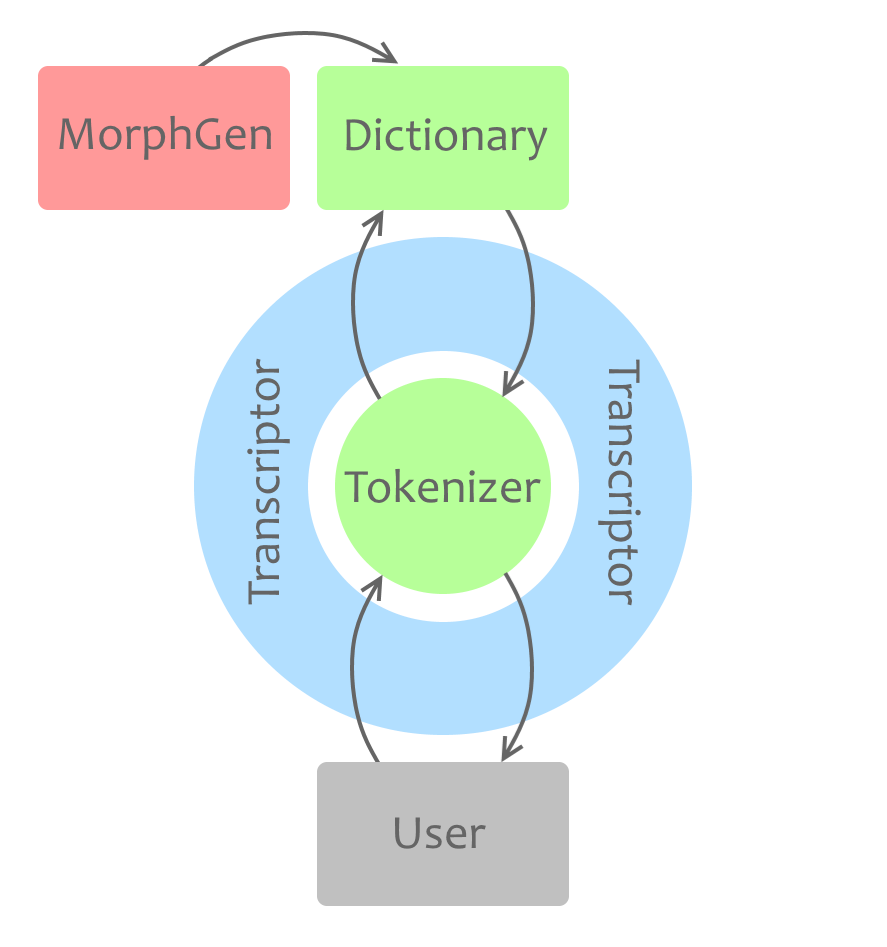
\includegraphics[width=0.5\textwidth]{systemarchitecture.png}
\caption{The architecture of the Malayalam Glosser.}
\label{architecture}
\end{figure}

The architecture of the system is illustrated in Figure \ref{architecture}. The heart of the program, the tokenizer, receives input from the user which it attempts to split into units that can be found in the dictionary. The entries in the dictionary are provided by the morphological generator. A transcriptor converting between different representations of Malayalam is wrapped around the tokenizer to make sure that the input and output are in the format desired by the user and the dictionary.

The Malayalam Glosser and all of its modules have been written in Java. The web interface was created using the GWT-Bootstrap library \parencite{gwtbootstrap}.

The following sections elaborate the workflow of the individual parts of the Malayalam Glosser in more detail, starting with the transliterator, then turning towards the morphological generator and the resulting dictionary, and finally elaborating the actual tokenization and glossing process.

\subsection{Transliteration}

Due to its syllabic nature, morpheme splitting is a tedious task in the Malayalam script and is best carried out in an alphabetic transcription. Also, while the Malayalam script has been included in Unicode for quite some time and Malayalam keyboard layouts are preinstalled on most modern machines, even native speakers of Malayalam frequently type Malayalam in a Latin romanization. Language learners, the primary target audience of the Malayalam Glosser, often do not know how to use the Malayalam script on a computer, especially when they are beginners. It is therefore necessary to convert Malayalam text between the script and various romanizations to be able to support the most popular input formats and display the finished glosses in a readable way.

\subsubsection{Supported Scripts}\label{scripts}

Apart from the Malayalam script, the Malayalam Glosser currently supports two additional romanization schemes, Mozhi and ISO-15919. The Mozhi romanization is very popular especially among Malayalis to write Malayalam on the web. It consists only of ASCII characters and utilizes capitalization to enlarge the set of available characters \parencite{mozhi}. The ISO-15919 or National Library at Kolkata romanization is the default romanization scheme in scientific texts for all Indic languages (it is also the one used in this paper). It makes heavy use of diacritics and is thus not easily typable on the average English keyboard. Because of this, there also is an ASCII version of ISO-15919 which replaces the diacritics by punctuation characters \parencite{iso-15919}. Both variants of ISO-15919, Unicode and ASCII based, are supported by the Malayalam Glosser.

A full table with all Malayalam characters in the different scripts (Malayalam script, Unicode ISO-15919, ASCII ISO-15919 and Mozhi) can be found in the appendix. (\ref{supportedScripts}) is an example of how the sentence `all human beings are born free and equal in dignity and rights' is spelled in the four supported scripts \parencite{malOmniglot}.

\ex
\textbf{Malayalam:} മനുഷ്യരെല്ലാവരും തുല്യാവകാശങ്ങളോടും അന്തസ്സോടും സ്വാ\-ത\-ന്ത്ര്യ\-ത്തോ\-ടും\-കൂ\-ടി ജനിച്ചവരാണ്. \\[1ex]
\textbf{Unicode ISO-15919:} manuṣyarellāvaruṁ tulyāvakāśaṅṅaḷōṭuṁ antassōṭ\-uṁ svātantryattōṭuṁkūṭi janiccavarāṇŭ. \\[1ex]
\textbf{ASCII ISO-15919:} manu.syarellaavaru;m tulyaavakaa;sa;n;na.loo.tu;m antassoo.t\-u;m svaatantryattoo.tu;mkuu.ti janiccavaraa.n\^{}u. \\[1ex]
\textbf{Mozhi:} manushyarellaavarum thulyaavakaaSangngaLOTum anthassOT\-um svaathanthryaththOTumkuuTi janichchavaraaN\textasciitilde{}.
\label{supportedScripts}\xe

The ASCII ISO-15919 romanization is also the underlying representation of all dictionary entries, since the Malayalam rules of the morphological generator are written in this format.

\subsubsection{Transliterators}

The main class handling all transliterations between the different scripts is the \typ{MalayalamTranscriptor}. However, it mostly serves as an interface to the transliterator system designed for the NorthEuraLex database by the EVOLAEMP project \parencite{northeuralex}. To display phonetic transcriptions for the lexical entries in their database, they developed automatic rule-based transliterators that are able to convert from orthography to IPA based on language-specific rule sets \parencite{daneyko2016translit}. Since phonetic transcription is just another type of transliteration, the same infrastructure can also be used to convert between different romanization schemes. The EVOLAEMP transliterators also have an efficient FST based implementation, the Java version of which is quite platform-dependent, so the basic Java implementation (called `simple transliterators' in \textcite{daneyko2016translit}) was used in a slightly altered form.

Transliterator rules from Malayalam script to Unicode ISO-15919 and from Unicode ISO-15919 to IPA were already written for the NorthEuraLex database. Hence, Unicode ISO-15919 was selected as the intermediate representation for the transliterators and additional rules were written for Unicode ISO-15919 to Malayalam script, Unicode ISO-15919 from and to ASCII ISO-15919, and Unicode ISO-15919 from and to Mozhi.


\subsection{Morphological generation}

The morphological generator, \typ{MorphGen}, is a standalone module responsible for generating the fully inflected paradigms of a lemma. It is based on user-provided rule sets and is thus not specialized on Malayalam, but can serve as a morphological generator for any language. Though its rules look similar to regular expressions and are interpreted by an automaton-like structure, \typ{MorphGen} is not a finite state transducer. Its ability to store matches in memory and freely reinsert them later allows it to easily model morphological processes that are inherently difficult to express with a finite state machine, such as reduplication and metathesis.

The \typ{MorphGen} rule set for Malayalam currently covers the grammar from lessons 1 to 13 from the \textcite{moag} text book.

\subsubsection{File format}

\begin{figure}[t]
\centering
\begin{tabular}{>{\ttfamily}l >{\ttfamily}l}
{}[*]\ci{}u|DAT & [1]|in\ci{}u \\
{}[*]u|DAT & [1]u|vin\ci{}u \\
{}[*];m|DAT & [1]tt|in\ci{}u \\
{}[*][!. \_]l|DAT & [1][2]l|kk\ci{}u \\
{}[*][!l r]|DAT & [1][2]|in\ci{}u \\
{}[*]n|DAT & [1]n|\ci{}u \\
{}[*]|DAT & [1]|kk\ci{}u \\
\end{tabular}
\caption{The dative rules from the Malayalam \typ{MorphGen} rule set.}
\label{dative-rules}
\end{figure}

\typ{MorphGen} requires one file containing the rules for generating the inflected words from a given gloss. The rule file is a simple text file, with one rule per line, input and output side of each rule separated by a tab stop. Figure \ref{dative-rules} shows an excerpt from the Malayalam rule file.

Since some scripts, notably the ASCII ISO-15919 romanization for Malayalam, may use the \typ{-} and \typ{.}\ characters that are usually displayed in glosses, \typ{MorphGen} operates on \typ{|} and \typ{\&} instead. Hence, the gloss `mouse.\afx{pl}-\afx{gen}' would be written \typ{mouse\&PL|GEN} in the \typ{MorphGen} format. For infixes, \typ{<>} is used (e.g.\ \typ{mouse<>PL|GEN}).

A couple of special characters can be used inside rules for easier matching:

\begin{itemize}
\item{} \typ{[*]} is a wildcard matching any number (including none) of characters. The matched characters can be referred to on the output side by an integer corresponding to the position of the wildcard on the left side. Applying the rule \typ{[*]x[*]y[*] \arr x[3][2]z[2]} to the input \typ{aaxbyccc}, for example, would assign \typ{aa} to 1, \typ{b} to 2 and \typ{ccc} to 3 and hence produce the output \typ{xcccbzb}. These wildcards can also be named and referred to by their name on the right side, as in \typ{[*]x[name]y[*] \arr x[2][name]z[name]}. Note that these names do not increase the counter for the wildcard labels: The variable previously referred to as 3 on the right side is now labeled 2.

\item By default, \typ{MorphGen} inserts wildcards at the beginning and end of the string if not present and matches them once at the beginning and end on the right side. The rule \typ{a \arr b} gets translated to \typ{[*]a[*] \arr [1]b[2]}, for example. To prevent this, word boundaries may explicitly be matched by a hash tag \typ{\#} on the left side. Thus, the rule \typ{a\# \arr b} will be converted to \typ{[*]a \arr [1]b}, matching only \typ{a}s at the end of a string.

\item A frequently recurring group of characters to match can be defined on top of the file using the keyword \typ{\#def} followed by the variable name followed by the group contents in square brackets, as in \typ{\#def \tab \#V \tab [aa ai au ee ii oo uu a e i o u]} which defines the set of vowels in Malayalam. Note that the \typ{\#def} keyword, the group name and the group definition are tab separated, while the strings inside the group definition are separated by whitespaces. The name of a group variable must always begin with a hash tag \typ{\#} to distinguish it from the named wildcards. These groups can be referenced on the left side of a rule with \typ{[\#name]} and on the right side with their integer label just like wildcards, as in \typ{[*][\#V]t[\#V][*] \arr [1][2]d[3][4]}.

\item Ad-hoc groups for a single rule may be created with \typ{[!item1 item2 ...]}, as in the example in Figure \ref{dative-rules}.

\item An optional group, i.e.\ a group matching one or none of the contained characters can be introduced with \typ{[?item1 item2 ...]}. Predefined groups may also be optionalized by referring to them with \typ{[?\#name]}. Consider for example the rule \typ{\#[?\#C][\#V].tuka|PST \arr [1][2].t|.tu} used to produce the past tense form of Malayalam verbs of the type (C)V\textit{ṭuka}. The optionally matched initial consonant is reprinted in the \typ{[1]} position on the right side only if it was actually found.

\item Sometimes the realization of same form may differ between words. For instance, the past tense of the verb വിൽക്കുക \textit{vilkkuka} `to sell' is \textit{viṟṟu}, while that of നിൽക്കുക \textit{nilkkuka} `to stand' is \textit{ninnu}. The phonological cues for selecting the appropriate past tense form have long been lost on these verbs, hence to get a complete paradigm, we may want to generate both forms. Multiple output sides for a single input side are separated by \typ{||}, as in this past tense rule for verbs ending in \textit{-lkkuka}: \typ{[*]lkkuka|PST \arr [1]\_r|\_ru || [1]n|nu}.
\end{itemize}

\label{parfile}\typ{MorphGen} optionally requires a second file specifying the templates for paradigm generation (see section \ref{pargen}). In this file, the possible inflections for each part of speech and the order in which they may occur are defined in a regular expression-like notation. This is the specification for Malayalam nouns:

\typ{[n] PL (NOM || ACC || DAT || GEN || SOC || INS || LOC)}

This means that a Malayalam word labeled with the part of speech tag \typ{n} can optionally have the feature \typ{PL}, optionally followed by any of the case features. It spells out as: \typ{n}, \typ{n PL}, \typ{n PL NOM}, \typ{n NOM}, \typ{n PL ACC}, etc. A whitespace is used to separate two features or feature groups that optionally occur in this order. \typ{||} means `or'. The whitespace takes precedence over the `or' operator, hence the case labels in the above have to be grouped together by parentheses.

This is part of the specification for Malayalam verbs (the actual one is much larger and more complex):

\typ{[v] PASS (((PRS || PST) (Nn || Nm || Nf) || PST\_STAT) (NEG || A)}

Here, a verb can (optionally) take the passive (\typ{PASS}). This may (optionally) be followed by either the present/past tense (\typ{PRS || PST}) and (optionally) a nominalizer (\typ{Nn || Nm || Nf}), or the past tense obligatorily followed by the stative perfect marker \textit{iṭṭŭ} (\typ{PST\_STAT}). Finally, the verb can (optionally) either be negated or adjectivized (\typ{NEG || A}). Note that the underscore \typ{\_} is used to delete the optionality of the whitespace and force the two features to occur together. The above rule will produce \typ{v} and \typ{v PST STAT} (and \typ{v PST} due to the earlier mentioning of \typ{PST}), but not \typ{v STAT}.

\subsubsection{Automated inflection}

One task of \typ{MorphGen} is the generation of the inflected form of a word according to its feature tags in the \typ{generate} method. The input \typ{kaa.nuka|PRS|NEG}, for example, will produce the morpheme-split negated present tense form of the verb \textit{kāṇuka} `to see', \typ{kaa.n|unn|illa}.

\begin{figure}
\begin{tikzpicture}[shorten >=2pt,node distance=1.5cm,auto] 
\node[state,initial] (0) {0};
\node[state] (1) [right=of 0] {1};
\node[state] (2) [right=of 1] {2};
\node[state] (3) [right=of 2] {3};
\node[state,accepting] (4) [right=of 3] {4}; 
\path[->] 
(0) edge[bend left] node {\typ{c $\in$ \#C \arr 1}} (1)
(0) edge[bend right] node[below] {\typ{$\varepsilon$ \arr 1}} (1)
(1) edge[bend right] node[below] {\typ{v $\in$ \#V \arr 2}} (2)
(2) edge[bend left] node {\typ{.tuka|PST}} (3)
(3) edge[bend right] node[below] {\typ{* \arr 3}} (4);
\end{tikzpicture}
\caption{The automaton representing the left side of the rule \typ{\#[?\#C][\#V].tuka|PST \arr [1][2].t|.tu} (converted to \typ{[?\#C][\#V].tuka|PST[*]} before).}
\label{morphrule}
\end{figure}

To achieve this, \typ{MorphGen} stores the rules specified in the rule file as a automaton-like representation and applies them in the order in which they are listed in the file. This means that the output of each rule serves as the input to the next one. Figure \ref{morphrule} illustrates the structure of such a rule automaton for the past tense rule for (C)V\textit{ṭuka} verbs discussed in the previous section.

Given an input such as \typ{i.tuka|PST|Nn} `to drop', \typ{MorphGen} will attempt to reach the final state of the rule while matching the characters of the input against the labels of the transitions and saving matched characters to variables where applicable. In this example, the start state of the rule has outgoing transitions for each of the characters in the \typ{\#C} group and an epsilon transition matching the empty string, because the match is optional. Since \textit{iṭuka} starts with a vowel, none of the \typ{\#C} transitions apply and the rule will take the epsilon transition, saving the empty string to the variable \typ{1}. To reach the next state, it must match a member of the \typ{\#V} group. Luckily, the current character, \typ{i}, satisfies this condition and is saved to the variable \typ{2}. Left with the string \typ{.tuka|PST|Nn}, the rule can take the literal transition \typ{.tuka|PST}. The final transition is a wildcard, consuming the remaining string \typ{|Nn} and saving it to the variable \typ{3}. The final state is reached and the string is accepted.

Now the output will be generated by unfolding the right hand side of the rule, \typ{[1][2].t|.tu[3]}. Here, \typ{MorphGen} simply inserts the values saved to the different variables, yielding the output string $\varepsilon$ + \typ{i} + \typ{.t|.tu} + \typ{|Nn} = \typ{i.t|.tu|Nn} which can now serve as the input to the next rule. If a string is not accepted by a rule in the first place, it will remain unaltered. If there are still feature tags (such as \typ{PST} or \typ{Nn}) left in the output after all rules have been applied, it is considered to be ungrammatical and discarded.

\subsubsection{Paradigm generation}\label{pargen}

The second task of \typ{MorphGen} is the generation of all possible glossed or feature tagged forms of a word in the \typ{getParadigm} method. In principle, this simply means spelling out all possible inflection tags that are specified for the word's part of speech in the paradigm template file (see section \ref{parfile}). Hence, given e.g.\ the word \textit{pūcca} `cat' and the part of speech tag \typ{n}, the paradigm generator will return the strings \typ{puucca}, \typ{puucca PL}, \typ{puucca PL GEN}, \typ{puucca GEN}, \typ{puucca PL ACC}, etc. These can now serve as input to the inflection rules.

When given a string such as \typ{puucca GEN}, \typ{MorphGen} will first fill the whitespaces between the feature tags with the separators \typ{|}, \typ{\&} and \typ{<>}. Hence, \typ{puucca GEN} will first be converted to the three strings \typ{puucca|GEN}, \typ{puucca\&GEN} and \typ{puucca<>GEN}. The latter two will hopefully not be matched by any rule and thus be sorted out as ungrammatical, while the first one can be realized as \typ{puucca|yu.te}, serving as the only possible output for \typ{puucca GEN}.

The two steps are combined in the \typ{getInflections} method, which accepts a word and a part of speech tag, e.g.\ \typ{puucca} and \typ{n}, and returns all possible inflections and glosses of that word (\typ{puucca puucca}, \typ{puucca|GEN puucca|yu.te}, \typ{puucca|PL|GEN puucca|ka.l|u.te}, \typ{puucca|ACC puucca|ye}, etc.). Finally, a whole vocabulary list can be given to the \typ{unfoldVocabulary} method to get a file with all inflected forms of all words in that list.


\subsection{Dictionary lookup}

The fully inflected dictionary provided by \typ{MorphGen} is handled by the \typ{MalayalamDictionary} class. Given a raw word (such as \typ{vii.tuka.lil}), it will return the matching morpheme-split string (\typ{vii.tu|ka.l|il}) and glosses (\typ{house|PL|LOC} and \typ{home|PL|LOC}). It is also able to carry out a suffix search on a string, returning the start index of the longest suffix found in the dictionary. For \typ{aavii.t.til} (\textit{ā} `that' + \textit{vīṭṭil} `house-\afx{loc}'), for example, it will return 2, since the longest known suffix, the inflected word \typ{vii.t.til}, starts at index 2.

In addition to the free morpheme classes (nouns, verbs, etc.), the dictionary also stores clitics, most prominently the question particle \textit{ō}, since they can attach to multiple (or even all) parts of speech. This means that they will be split off by the tokenizer just like any other token in the dictionary.

In its current version, the dictionary knows 15,015 inflected forms generated from 279 lemmas obtained from the vocabulary lists from lessons 1 to 11 from the \textcite{moag} text book. Thus, the Glosser's vocabulary is currently still quite small, but it will be extended in the future.

\subsubsection{Efficiency considerations}

Considering that the dictionary may be very large and that the main function of the Glosser is to look words up in this dictionary, being able to load and query it very fast is essential for the performance of the Glosser. Hence, I experimented with a few alternatives for storing the dictionary data and investigated their efficiency. The tests elaborated below are not very thorough and were only meant to quickly assess the usefulness of the considered methods.

\subsubsection*{\typ{HashMap} vs. \typ{ReverseTrie}}

The straightforward way to represent a dictionary as a Java object is a \typ{HashMap}. Apart from being readily available and easy to use, querying a \typ{HashMap} is fast. However, this also means that all entries are stored as their complete \typ{String} representation, which may consume quite a lot of space. Considering that the inflected forms of the words share most of their characters, a trie representation seemed quite suitable and might be able to save space compared to a simple \typ{HashMap}. Since Malayalam is exclusively suffixing, I programmed a \typ{ReverseTrie} which reads and retrieves the strings from last to first character, in order to save as much space as possible. A useful side effect of this is that the \typ{ReverseTrie} comes with a natural suffix search method and the dictionary does not need to look up all possible suffixes of a compound word to find the longest suffix.

In order to compare the performance of a \typ{HashMap} and \typ{ReverseTrie} based dictionary, I measured the memory used by the program before loading the dictionary data and after creating the \typ{HashMap} and \typ{ReverseTrie} (calculated as \typ{Runtime.totalMemory() - Runtime.freeMemory()} after a \typ{System.gc()} call). Then I let the dictionary find the longest known suffix of the test String \textit{aviṭeyuḷḷataṟiññu} (\textit{aviṭe uḷḷatŭ aṟiññu} ``knew (he) was there'') 1,000,000 times and measured the time needed by a \typ{HashMap} and \typ{ReverseTrie} based dictionary (calculated using \typ{System.currentmillis()}). Finally, I rewrote the suffix search method to also work with a \typ{ReverseTrie} and tested how long tokenization of the short conversation from lesson 11 of \textcite[p.164f, see appendix]{moag} took with the two dictionary types.

Despite the many shared suffixes, the \typ{HashMap} was smaller than the \typ{ReverseTrie}, taking up 8,318,164.8 bytes on average during five test runs, while the \typ{ReverseTrie} required 12,590,051.2 bytes. However, the memory used by the \typ{HashMap} varied greatly, ranging from only 5,160,456 to 9,801,392 bytes, while the \typ{ReverseTrie} always consumed almost exactly the same amount of memory. This indicates that the measurements might have been distorted by background processes such as the garbage collection. However, the \typ{HashMap} still seems to be considerably smaller.

As expected, the \typ{ReverseTrie} outperformed the \typ{HashMap} on the looped suffix search of \textit{aviṭeyuḷḷataṟiññu}. The \typ{HashMap} took an average of 999 milliseconds during five test runs, while the \typ{ReverseTrie} only needed 312.4 ms. However, the performance of the \typ{ReverseTrie} was very unstable, ranging from 140 to 518 ms between runs, while the \typ{HashMap} always needed between 908 and 1049 ms, which is still much slower than the slowest suffix search of the \typ{ReverseTrie}.

On a real Malayalam text, where only few words are long compounds such as \textit{aviṭeyuḷḷataṟiññu}, both methods were equally fast. During 10 glossings of the Moag conversation, the \typ{HashMap} based tokenization took 156.3 ms on average and the \typ{ReverseTrie} based tokenization 161.7 ms. Both ran very stable.

All in all, the \typ{HashMap} seems to be the better choice, since it is smaller than the \typ{ReverseTrie} and equally fast on normal Malayalam texts. The \typ{ReverseTrie} is faster when tokenizing long compound words, which however are not frequent enough to justify preferring it over the \typ{HashMap}.

\subsubsection*{File storage vs. Serialization}

Loading the dictionary data into the underlying \typ{HashMap} (or \typ{ReverseTrie}) takes a considerable amount of time at launch. Hence, I considered serializing the Map or Trie object to be able to load it quicker. Since the Java serialization is known to be rather slow, I used the FST Fast Serialization library \parencite{fastSerialization} for my tests. I first read the dictionary data from the text file and created the \typ{HashMap} and \typ{ReverseTrie} from it, measuring the time needed. Then I serialized the two objects and took the time required to deserialize them.

During five test runs, parsing the text file into an object took 278.2 ms on average for the \typ{HashMap} and 310.6 ms for the Trie. Deserializing the same objects required 563.4 ms on average for the \typ{HashMap} and 339.8 ms for the Trie. Loading the data from a text file is thus faster than deserializing a previously created object.

The file storing the serialized \typ{ReverseTrie} was twice as large as the file with the \typ{HashMap}. This confirms my assertions from the previous section that the Trie takes more space than the \typ{HashMap}.


\subsection{Tokenization and Glossing}

The core of the system is the \typ{MalayalamGlosser} which handles both the tokenization and glossing of the input text with the help of the \typ{MalayalamTranscriptor} and \typ{MalayalamDictionary} classes.

Given an input text, it will first split it into individual sentences using a simple regular expression that matches punctuation characters. For each sentence, it will then perform a simple whitespace tokenization. The resulting `rough' tokens are then converted to the ASCII ISO-15919 format that is used by the dictionary and handed to the sandhi splitter.

The sandhi split method recursively does a suffix search in the dictionary to remove the final token from the word. The remaining prefix of the string is then checked against a range of sandhi rules to generate candidate strings for the next sandhi split. One candidate is always the unmodified string. Then, if for example the prefix ends in a glide (\textit{y} or \textit{v}) and the recognized suffix starts with a vowel, another candidate is the prefix without the final glide, since it might have been subject to glide insertion. If at some point the prefix is empty, the string was successfully tokenized. If it could not be split into tokens in this way, i.e.\ if no valid candidate could be generated for a prefix, it will be tagged as \typ{<unknown>}. Of course, this means that if any of the tokens in the string is not known to the dictionary, the whole compound will be marked as unknown and is not split.

The identified tokens of each sentence are finally looked up in the dictionary and tagged with their possible morpheme splits and glosses in the selected output script as well as provided with a phonetic transcription in IPA. Also, since the original word might have been split into several tokens, each token is converted back from the dictionary format (ASCII ISO-15919) to the original input script.


\section{Evaluation}\label{sec:eval}

\subsection{MorphGen}

\subsubsection{Expressivity of the rule format}

Malayalam served as the first test case for \typ{MorphGen} to see whether the developed rule format would be expressive enough to cover an agglutinative morphology. The results are very satisfying: Only 202 rules were sufficient to cover all of the grammar from the first 13 \textcite{moag} lessons which already introduce the most common Malayalam morphology. Also, 39 of these rules are exceptions (such as the first and second person singular pronouns) and 47 rules belong the number generator spelling out the numerals from one to 900 in Malayalam. Thus, we are left with 116 rules covering the regular grammar including all \textit{internal sandhi} processes.

However, designing the Malayalam rules also revealed a few issues and missing features. First of all, a literal string in a rule also matches all intervening separators (\typ{|}, \typ{\&}, \typ{<>}) to be able to apply a rule such as \typ{[*]xy|FOO \arr [1]xy|abc} to an input such as \typ{xxxx|y|FOO}, where \typ{y} is a suffix generated by a previous rule. However, the exact match of a literal like \typ{xy|FOO} (which would be \typ{x|y|FOO} in this case) is not saved like a variable, because it is not referenced on the other side. Instead, the literal \typ{xy|abc} is attached to the output. Hence, \typ{xxxx|y|FOO} will be converted to \typ{xxxxy|abc}, losing the separator from the previous rule and thus resulting in an incomplete gloss. At \typ{MorphGen}'s current stage, such matches must be kept in mind and accounted for by writing the rules as \typ{[*]x[?|]y|FOO \arr [1]x[2]y|abc}, which is not feasible as the covered grammar grows.

Another problem is that the separators that are randomly placed at whitespaces between feature tags by the paradigm generator (e.g.\ realizing \typ{puucca PL} as \typ{puucca<>PL}) sometimes lead to the creation of false forms. Even though Malayalam is exclusively suffixing, the paradigm will always create glosses containing infix separators (\typ{<>}). These are supposed to be sorted out because no rules can apply to them. However, the rules sometimes do not explicitly match the appropriate separator (such as \typ{|}), but only the feature tag itself (such as \typ{PL}). In this case, all features will be realized and the incorrect gloss apparently containing an infix will end up in the generated paradigm. A way to explicitly mark these forms as false and remove them from the candidate pool would be very useful. Currently, the only way to achieve this is to write a rule that inserts feature tags into unwanted words that cannot be resolved anymore by the following rules. For example, there is a rule in the Malayalam file below the part covering negation that transforms all infix separators into the \typ{NEG} tag. Since there is no following rule matching this tag anymore, the word will be rejected by the paradigm generator since it looks as if it contains a feature that couldn't be matched. This must of course only be a temporary workaround. Simply being able to place a rule like \typ{<> \arr REMOVE} at the beginning of a file that states `all inputs containing \typ{<>} are illegal' is a necessary addition to the \typ{MorphGen} language.

Finally, a negation group operator that states `match if not followed by any of these characters' could prove useful and would be easy to implement.

\subsubsection{Performance}

The big drawback of \typ{MorphGen} is the sheer size of a completely inflected vocabulary, especially for a morphologically rich language like Malayalam. While a single noun has `only' 21 to 22 forms (depending on whether the phonology of the word allows for an alternative locative form), a verb generates around 195 forms; and these numbers are still going to multiply as the full grammar of Malayalam is implemented.

Single forms and lemmas may be generated quickly, but unfolding a larger vocabulary list takes very long. The original plan for the Malayalam Glosser was to use the complete Olam English-Malayalam dataset \parencite{olam} as the underlying dictionary, which contains over 200,000 English words with Malayalam translations and definitions. After reversing the translation direction from English-Malayalam to Malayalam-English, removing all Malayalam multi-word entries (i.e.\ those containing whitespaces) and transliterating the Malayalam words to ASCII ISO-15919, the list contained 67,461 unique Malayalam words with English translations. However, unfolding this list with \typ{MorphGen} was cancelled after it had run for almost seven hours. At this point, it had only consumed 68 \% of the Malayalam entries but already generated 6 million inflected forms.

After adjusting the output file format to reduce the size of the generated file, I ran \typ{MorphGen} over a subset of 6,329 verbs from the Olam database. These were successfully unfolded into 1,521,859 forms in roughly 4.5 hours. However, loading the resulting dictionary into the Malayalam Glosser took several minutes before the program threw an `Out of memory' error. The fully inflected Olam database is thus far too large to be handled by the Malayalam Glosser.

\subsection{Malayalam Glosser}

Evaluating the Malayalam Glosser itself is difficult, because its performance is largely dependent on the size of the vocabulary provided by the \typ{MorphGen} module. Currently, it is only usable for texts from the \textcite{moag} text book, as the dictionary only contains lexical items from the book. However, since even the grammar is geared to the Moag lessons, good performance on the Moag texts is already guaranteed. Hence, the Glosser still needs to be extended both in terms of vocabulary and grammar until it can be properly applied to and evaluated with arbitrary texts.

Its exemplary output for the Moag conversation from lesson 11 can be viewed in the appendix.


\section{Outlook}

In this paper, I have presented an automatic glosser for Malayalam that is theoretically able to generate interlinear glosses for an arbitrary Malayalam text, providing valuable grammatical and lexical information to a user seeking to understand the structure and meaning of that text. In its current version, the functionality of the Malayalam Glosser is unfortunately still severely limited by its small vocabulary. Generating a larger vocabulary is difficult since the glosser relies on a morphology generator and Malayalam's morphology is so complex that a fully inflected vocabulary is unreasonably large.

Therefore, it seems inevitable to use a morphological analyzer instead of a morphological generator to analyze the inflected forms occurring in the user submitted texts. It should be possible to implement morphological analysis on top of the existing \typ{MorphGen} module by reversing the rules written for morphological generation, i.e.\ going from inflected to tagged words and then looking the generated root forms up in the dictionary. Once the rules have been reversed, they should be applicable using the already established automaton-based infrastructure.

With a morphological analyzer at hand, the vocabulary of the Malayalam Glosser should be easily extendable to e.g.\ the Olam database \parencite{olam}. Once the full grammar of Malayalam, as e.g.\ described in \textcite{asherKumari}, is implemented, the Glosser should be able to operate on arbitrary contemporary texts, representing a powerful aid in Malayalam language learning.


\printbibliography
\clearpage

\appendix

\section{Abbreviations used in glosses}

These are the abbreviations used in the glosses of sections \ref{sec:intro} and \ref{sec:malnlp}. A list of the abbreviations used by the Malayalam Glosser can be found on the Help page of the application.

\begin{multicols}{2}
\begin{labeling}{XXXX}
\itemsep0em
\item [\textsc{cau}] Causative
\item [\textsc{cop}] The copula \textit{āṇŭ}
\item [\textsc{dat}] Dative case
\item [\textsc{des}] Desiderative mood
\item [\textsc{pass}] Passive voice
\item [\textsc{perf}] Perfect aspect
\item [\textsc{pl}] Plural number
\item [\textsc{prog}] Progressive aspect
\item [\textsc{prs}] Present tense
\item [\textsc{pst}] Past tense
\item [\textsc{part}] Participle
\item [\textsc{soc}] Sociative case
\end{labeling}
\end{multicols}

\section{Transcription schemes}

This is a list of the Malayalam characters in the four supported scripts of the Malayalam Glosser as outlined in section \ref{scripts}.

\begin{longtable}[l]{p{2.3cm} p{2.3cm} p{2.3cm} p{2.3cm}}
\textbf{Script} & \textbf{ISO (Uni)} & \textbf{ISO (ASCII)} & \textbf{Mozhi} \\[1ex]
അ & a & a & a \\
ആ & ā & aa & aa \\
ഇ & i & i & i \\
ഈ & ī & ii & ii \\
ഉ & u & u & u \\
ഊ & ū & uu & uu \\
ഋ & \ipa{r̥} & ,r & R \\
എ & e & e & e \\
ഏ & ē & ee & E \\
ഐ & ai & ai & ai \\
ഒ & o & o & o \\
ഓ & ō & oo & O \\
ഔ & au & au & au \\
അം & aṁ & a;m & am \\
അഃ & aḥ & a.h & ah \\
ക & ka & ka & ka \\
ഖ & kha & kha & kha \\
ഗ & ga & ga & ga \\
ഘ & gha & gha & gha \\
ങ & ṅa & ;na & nga \\
ച & ca & ca & cha \\
ഛ & cha & cha & chha \\
ജ & ja & ja & ja \\
ഝ & jha & jha & jha \\
ഞ & ña & \textasciitilde{}na & nja \\
ട & ṭa & .ta & Ta \\
ഠ & ṭha & .tha & Tha \\
ഡ & ḍa & .da & Da \\
ഢ & ḍha & .dha & Dha \\
ണ & ṇa & .na & Na \\
ത & ta & ta & tha \\
ഥ & tha & tha & thha \\
ദ & da & da & da \\
ധ & dha & dha & dha \\
ന & na & na & na \\
പ & pa & pa & pa \\
ഫ & pha & pha & pha \\
ബ & ba & ba & ba \\
ഭ & bha & bha & bha \\
മ & ma & ma & ma \\
യ & ya & ya & ya \\
ര & ra & ra & ra \\
ല & la & la & la \\
വ & va & va & va \\
ശ & śa & ;sa & Sa \\
ഷ & ṣa & .sa & sha \\
സ & sa & sa & sa \\
ഹ & ha & ha & ha \\
ള & ḷa & .la & La \\
ഴ & ḻa & \_la & zha \\
റ & ṟa & \_ra & rra \\
റ്റ & ṯṯa/ṟṟa & \_t\_ta/\_r\_ra & ta \\
ന്റ & nṯa/nṟa & n\_ta/n\_ra & nta \\
ൻ & n & n & n \\
ൺ & ṇ & .n & N \\
ർ & r & r & r \\
ൽ & l & l & l \\
ൾ & ḷ & .l & L \\
ൿ & k & k & k \\
ക് & kŭ & k\^{}u & k\textasciitilde \\
\end{longtable}

\section{Glossed translation of lesson 11 conversation}

The following is the complete conversation from lesson 11 (introducing the past tense, nominalization and cleft sentences with the copula \textit{āṇŭ}) of \textcite{moag} that I frequently used as a test input, as it was glossed by the Malayalam Glosser, translated by myself.

\ex\begingl
\glpreamble ചേച്ചി: അനിയൻ ആ മുറിയിൽ ആയിരുന്നല്ലോ. ഇപ്പോൾ അവനെ കാണുന്നില്ല. എവിടെ പോയി? \\
\itshape cēcci: aniyan ā muṟiyil āyirunnallō. ippōḷ avane kāṇunnilla. eviṭe pōyi?//
\gla അനിയൻ ആ മുറിയിൽ ആയിരുന്നല്ലോ . + ഇപ്പോൾ അവനെ കാണുന്നില്ല . + എവിടെ പോയി ? //
\glb aniyan ā muṟi-yil āyirun-n-allō . ippōḷ avan-e kāṇ-unn-illa . eviṭe pōy-i ? //
\glc younger\_brother that room-LOC temporarily\_be-PST-PAM . now he-ACC see-PRS-NEG . where go-PST ? //
\glft Older sister: `Younger brother used to be in that room. Now I don't see him. Where did he go?' //
\endgl\xe

\ex\begingl
\glpreamble അമ്മ: ഞാൻ അവനെ ചന്തയിൽ അയച്ചു. \\
\itshape amma: ñān avane cantayil ayaccu. //
\gla ഞാൻ അവനെ ചന്തയിൽ അയച്ചു . //
\glb ñān avan-e canta-yil ayac-cu . //
\glc I.NOM he-ACC market-LOC send-PST . //
\glft Mother: `I sent him to the market.' //
\endgl\xe

\ex\begingl
\glpreamble ചേച്ചി: ഓ! എന്തിനാണ് അയച്ചത്. \\
\itshape cēcci: ō! entināṇŭ ayaccatŭ. //
\gla ഓ ! എന്തിന് ആണ് അയച്ചത് . //
\glb ō ! ent-inŭ āṇŭ ayac-c-atŭ . //
\glc QPRT\footnotemark{} ! what-DAT COP send-PST-Nn . //
\glft Older sister: `Oh! Why is it that you sent him?' //
\endgl\xe

\footnotetext{This is of course not the question particle, but the interjection `oh', which is not contained in the dictionary.}

\ex\begingl
\glpreamble അമ്മ: ഇറച്ചി തീർന്നുപോയി. അത് വാങ്ങിക്കാനാണ് അയച്ചത്. \\
\itshape amma: iṟacci tīrnnupōyi. atŭ vāṅṅikkānāṇŭ ayaccatŭ. //
\gla ഇറച്ചി തീര്നനുപോയി . + അത് വാങ്ങിക്കാൻ ആണ് അയച്ചത് . //
\glb iṟacci tīrnnupōy-i . atŭ vāṅṅikk-ān āṇŭ ayac-c-atŭ . //
\glc meat run\_out-PST . that.ACC buy-GER COP send-PST-Nn . //
\glft Mother: `I ran out of meat. I sent him to buy that.' //
\endgl\xe

\ex\begingl
\glpreamble ചേച്ചി: അവൻ അതാ വരുന്നല്ലോ. ഇറച്ചി വാങ്ങിച്ചോ? \\
\itshape cēcci: avan atā varunnallō. iṟacci vāṅṅiccō? //
\gla അവൻ അത് ആണ് വരുന്നല്ലോ . + ഇറച്ചി വാങ്ങിച്ചു ഓ ? //
\glb avan atŭ āṇŭ var-unn-allō . iṟacci vāṅṅic-cu ō ? //
\glc he that COP come-PRS-PAM . meat.ACC buy-PST QPRT ? //
\glft Older sister: `There he comes. Did you buy meat?' //
\endgl\xe

\ex\begingl
\glpreamble അനിയൻ: വാങ്ങിച്ചു. പക്ഷെ, അത്ര നല്ലത് കിട്ടിയില്ല. \\
\itshape aniyan: vāṅṅiccu. pakṣe, atra nallatŭ kiṭṭiyilla. //
\gla വാങ്ങിച്ചു . + പക്ഷെ , അത്ര നല്ലത് കിട്ടിയില്ല . //
\glb vāṅṅic-cu . pakṣe , atra nall-atŭ kiṭṭ-i-yilla . //
\glc buy-PST . but , that\_many good-Nn find-PST-NEG . //
\glft Younger brother: `I did. But I didn't find that much good (meat).' //
\endgl\xe

\ex\begingl
\glpreamble ചേച്ചി: എന്തിനാണ് നീ ചീത്ത ഇറച്ചി കൊണ്ടുവന്നത്? \\
\itshape cēcci: entināṇŭ nī cītta iṟacci koṇṭuvannatŭ? //
\gla എന്തിന് ആണ് നീ ചീത്ത ഇറച്ചി കൊണ്ടുവന്നത് ? //
\glb ent-inŭ āṇŭ nī cītta iṟacci koṇṭuvan-n-atŭ ? //
\glc what-DAT COP you.NOM bad meat.ACC bring-PST-Nn ? //
\glft Older sister: `Why is it that you bring bad meat?' //
\endgl\xe

\ex\begingl
\glpreamble അനിയൻ: ഞാൻ ചന്തയിലെല്ലാം നോക്കി. നല്ല ഇറച്ചി ഇല്ലായിരുന്നു. \\
\itshape aniyan: ñān cantayilellāṁ nōkki. nalla iṟacci illāyirunnu. //
\gla ഞാൻ ചന്തയിൽ എല്ലാം നോക്കി . + നല്ല ഇറച്ചി ഇല്ലായിരുന്നു . //
\glb ñān canta-yil ellāṁ nōkk-i . nalla iṟacci illāyirunnu . //
\glc I market-LOC all look-PST . good meat be.PST.NEG . //
\glft Younger brother: `I looked everywhere on the market. There was no good meat.' //
\endgl\xe

\ex\begingl
\glpreamble ചേച്ചി: ഇതിന് എത്ര രൂപ കൊടുത്തു? \\
\itshape cēcci: itinŭ etra rūpa koṭuttu? //
\gla ഇതിന് എത്ര രൂപ കൊടുത്തു ? //
\glb it-inŭ etra rūpa koṭut-tu ? //
\glc this-DAT how\_many rupee.ACC give-PST ? //
\glft Older sister: `How many rupees did you pay for this?' //
\endgl\xe

\ex\begingl
\glpreamble അനിയൻ: പതിനഞ്ച് രൂപ. \\
\itshape aniyan: patinañcŭ rūpa. //
\gla പതിനഞ്ച് രൂപ . //
\glb patinañcŭ rūpa . //
\glc +1.*10.+5 rupee . //
\glft Younger brother: `Fifteen rupees.' //
\endgl\xe

\ex\begingl
\glpreamble ചേച്ചി: അയ്യോ! അത് വളരെ കൂടുതലാണല്ലോ. അത്രയും രൂപ വെറുതെ ക\-ള\-ഞ്ഞ\-ല്ലോ. \\
\itshape cēcci: ayyō! atŭ vaḷare kūṭutalāṇallō. atrayuṁ rūpa veṟute kaḷaññallō.//
\gla അയ്യോ ! അത് വളരെ കൂടുതൽ ആണല്ലോ . +  അത്രയും രൂപ വെറുതെ കളഞ്ഞല്ലോ . //
\glb ayyō ! atŭ vaḷare kūṭutal āṇ-allō . atrayuṁ rūpa veṟute kaḷañ-ñ-allō . //
\glc \textless{}unknown\textgreater{} ! that very\_much too\_much COP-PAM . as\_much\_as\_that rupee uselessly throw\_away-PST-PAM . //
\glft Older sister: `Oho! That is far too much. You threw away that many rupees for nothing.' //
\endgl\xe

\ex\begingl
\glpreamble അമ്മ: അതിന് നിനക്കെന്താ? പോകട്ടെ. എന്നാലും അത്ര ചീത്തയല്ല. കറി വെക്കാം. ചിലപ്പോൾ നന്നായിരിക്കും. \\
\itshape amma: atinŭ ninakkentā? pōkaṭṭe. ennāluṁ atra cīttayalla. kaṟi vekkāṁ. cilappōḷ nannāyirikkuṁ. //
\gla അതിന് നിനക്ക് എന്ത് ആണ് ? + പോകട്ടെ . + എന്നാലും അത്ര ചീത്ത അല്ല . + കറി വെക്കാം . + ചിലപ്പോൾ നന്ന് ആയിരിക്കും . //
\glb at-inŭ nin-akkŭ entŭ āṇŭ ? pōk-aṭṭe . ennāluṁ atra cītta alla . kaṟi vekk-āṁ . cilappōḷ nannŭ āyirikk-uṁ . //
\glc that-DAT you-DAT what COP ? go-PERM . anyway that\_many bad be.NEG . curry.ACC put-INT . perhaps good\_one temporarily\_be-FUT . //
\glft Mother: `Why do you care? It's okay. There isn't that much bad (meat) anyway. I will make curry. Perhaps it will be good.' //
\endgl\xe

\ex\begingl
\glpreamble ചേച്ചി: ഞാൻ കഴിക്കുകയില്ല. പട്ടിക്ക് കൊടുക്കാം. \\
\itshape cēcci: ñān kaḻikkukayilla. paṭṭikkŭ koṭukkāṁ. //
\gla ഞാൻ കഴിക്കുകയില്ല . + പട്ടിക്ക് കൊടുക്കാം . //
\glb ñān kaḻikk-ukayilla . paṭṭi-kkŭ koṭukk-āṁ . //
\glc I.NOM eat-INT.NEG . dog-DAT give-INT . //
\glft Older sister: `I'm not going to eat it. I'll give it to the dog.' //
\endgl\xe

\ex\begingl
\glpreamble അമ്മ: അങ്ങനെ പറയണ്ടാ, കേട്ടോ! നിനക്ക് അടി വേണോ? \\
\itshape amma: aṅṅane paṟayaṇṭā, kēṭṭō! ninakkŭ aṭi vēṇō? //
\gla അങ്ങനെ പറയണ്ട ആണ് , കേട്ടു ഓ ! + നിനക്ക് അടി വേണം ഓ ? //
\glb aṅṅane paṟay-aṇṭa āṇŭ , kēṭ-ṭu ō ! nin-akkŭ aṭi vēṇaṁ ō ? //
\glc that\_way speak-DES.NEG COP , hear-PST QPRT ! you-DAT spanking.NOM want.PRS QPRT ? //
\glft Mother: `You're not allowed to speak like that, did you hear! Do you want a spanking?' //
\endgl\xe

\end{document}